\begin{EXO}{Lecture graphique de paraboles}{}
\tcbitempoint{3} Pour chaque fonction représentée ci-dessous, déterminer les coordonnées du sommet, l'axe de symétrie et le signe de $a$.

\begin{MultiColonnes}{4}[boxrule=0.4pt,colframe=black]
\tcbitem[halign=center]
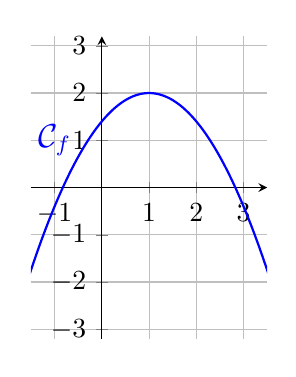
\begin{tikzpicture}
\begin{axis}[
x=1.0cm,y=1.0cm,scale=0.6,
axis lines=middle,
ymajorgrids=true,
xmajorgrids=true,
xmin=-1.5,
xmax=3.5,
ymin=-3.2,
ymax=3.2,
xtick={-1.0,0.0,...,3.0},
ytick={-3.0,-2.0,...,3.0},]
\clip(-1.5,-3.2) rectangle (3.5,3.2);
\addplot[thick,blue, samples=200] {-0.6*(x-1)^2+2};
\begin{scriptsize}
\draw[color=blue] (-1,1) node {\large{$\mathcal{C}_f$}};
\end{scriptsize}
\end{axis}
\end{tikzpicture}

Sommet : \tcfillcrep{$(1;2)$}

Axe : \tcfillcrep{$x=1$}
  
Signe de $a$ : \tcfillcrep{$a<0$}


\tcbitem[halign=center]
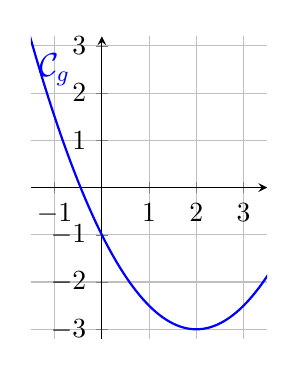
\begin{tikzpicture}
\begin{axis}[
x=1.0cm,y=1.0cm,scale=0.6,
axis lines=middle,
ymajorgrids=true,
xmajorgrids=true,
xmin=-1.5,
xmax=3.5,
ymin=-3.2,
ymax=3.2,
xtick={-1.0,0.0,...,3.0},
ytick={-3.0,-2.0,...,3.0},]
\clip(-1.5,-3.2) rectangle (3.5,3.2);
\addplot[thick,blue, samples=200] {0.5*(x-2)^2-3};
\begin{scriptsize}
\draw[color=blue] (-1,2.5) node {\large{$\mathcal{C}_g$}};
\end{scriptsize}
\end{axis}
\end{tikzpicture}

Sommet : \tcfillcrep{$(2;-3)$}

Axe : \tcfillcrep{$x=2$}
  
Signe de $a$ : \tcfillcrep{$a>0$}


\tcbitem[halign=center]
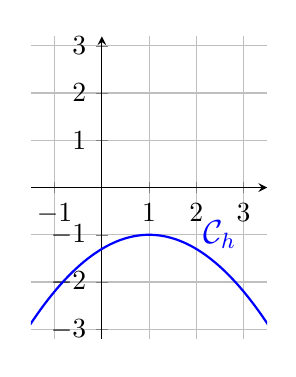
\begin{tikzpicture}
\begin{axis}[
x=1.0cm,y=1.0cm,scale=0.6,
axis lines=middle,
ymajorgrids=true,
xmajorgrids=true,
xmin=-1.5,
xmax=3.5,
ymin=-3.2,
ymax=3.2,
xtick={-1.0,0.0,...,3.0},
ytick={-3.0,-2.0,...,3.0},]
\clip(-1.5,-3.2) rectangle (3.5,3.2);
\addplot[thick,blue, samples=200] {-0.3*(x-1)^2-1};
\begin{scriptsize}
\draw[color=blue] (2.5,-1) node {\large{$\mathcal{C}_h$}};
\end{scriptsize}
\end{axis}
\end{tikzpicture}

Sommet : \tcfillcrep{$(1;-1)$}

Axe : \tcfillcrep{$x=1$}
  
Signe de $a$ : \tcfillcrep{$a<0$}


\tcbitem[halign=center]
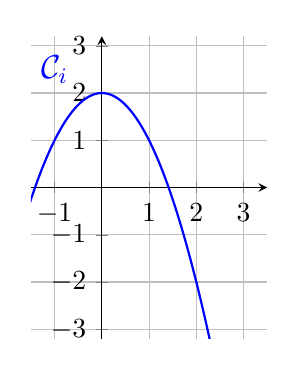
\begin{tikzpicture}
\begin{axis}[
x=1.0cm,y=1.0cm,scale=0.6,
axis lines=middle,
ymajorgrids=true,
xmajorgrids=true,
xmin=-1.5,
xmax=3.5,
ymin=-3.2,
ymax=3.2,
xtick={-1.0,0.0,...,3.0},
ytick={-3.0,-2.0,...,3.0},]
\clip(-1.5,-3.2) rectangle (3.5,3.2);
\addplot[thick,blue, samples=200] {-1*x^2+2};
\begin{scriptsize}
\draw[color=blue] (-1,2.5) node {\large{$\mathcal{C}_i$}};
\end{scriptsize}
\end{axis}
\end{tikzpicture}

Sommet : \tcfillcrep{$(0;2)$}

Axe : \tcfillcrep{$x=0$}
  
Signe de $a$ : \tcfillcrep{$a<0$}

\end{MultiColonnes}

\exocorrection

Pour chaque parabole, je lis graphiquement :

\begin{MultiColonnes}{4}
\tcbitem[halign=center] $\mathcal{C}_f$ : 
\begin{itemize}
\item Sommet au point le plus haut : $(1;2)$
\item Axe de symétrie vertical : $x=1$ 
\item Parabole vers le bas : $a<0$
\end{itemize}

\tcbitem[halign=center] $\mathcal{C}_g$ :
\begin{itemize}
\item Sommet au point le plus bas : $(2;-3)$
\item Axe de symétrie vertical : $x=2$
\item Parabole vers le haut : $a>0$
\end{itemize}

\tcbitem[halign=center] $\mathcal{C}_h$ :
\begin{itemize}
\item Sommet au point le plus haut : $(1;-1)$
\item Axe de symétrie vertical : $x=1$
\item Parabole vers le bas : $a<0$
\end{itemize}

\tcbitem[halign=center] $\mathcal{C}_i$ :
\begin{itemize}
\item Sommet au point le plus haut : $(0;2)$
\item Axe de symétrie vertical : $x=0$
\item Parabole vers le bas : $a<0$
\end{itemize}
\end{MultiColonnes}
\end{EXO}